\documentclass{standalone}
\usepackage{tikz}
\usetikzlibrary{patterns, positioning}


\begin{document}
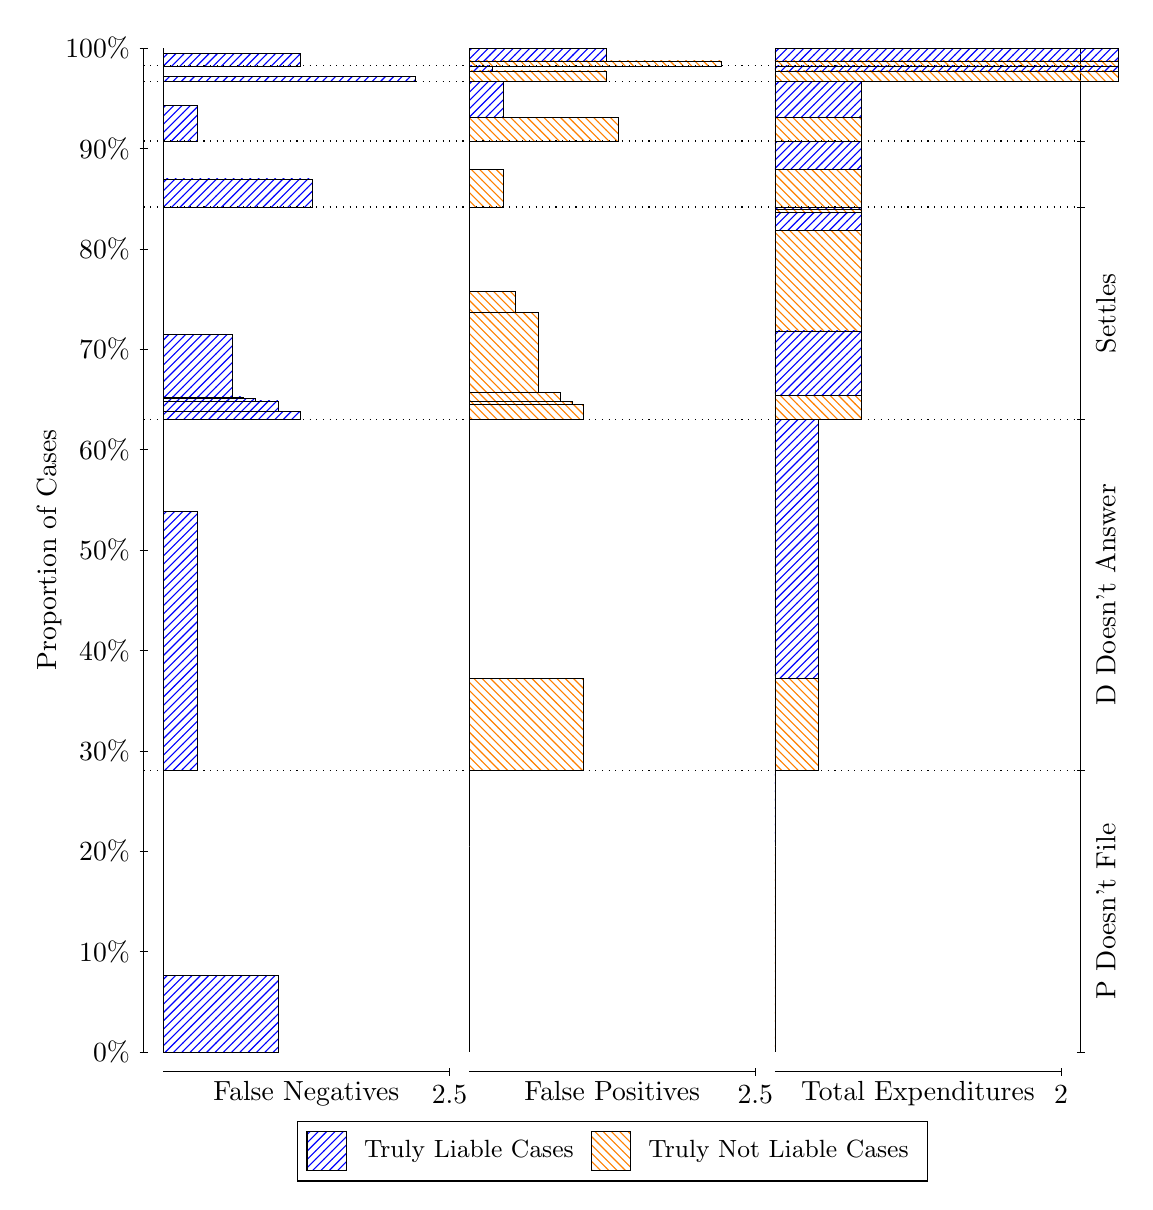
\begin{tikzpicture}
\draw[black, very thin] (1.5,1.75) -- (1.5,14.5);
\node[rotate=90, text=black, anchor=center] at (0.3, 8.125) {Proportion of Cases};
\draw[black, very thin] (1.45,1.75) -- (1.55,1.75);
\node[text=black, anchor=east] at (1.45, 1.75) {0\%};
\draw[black, very thin] (1.45,3.025) -- (1.55,3.025);
\node[text=black, anchor=east] at (1.45, 3.025) {10\%};
\draw[black, very thin] (1.45,4.3) -- (1.55,4.3);
\node[text=black, anchor=east] at (1.45, 4.3) {20\%};
\draw[black, very thin] (1.45,5.575) -- (1.55,5.575);
\node[text=black, anchor=east] at (1.45, 5.575) {30\%};
\draw[black, very thin] (1.45,6.85) -- (1.55,6.85);
\node[text=black, anchor=east] at (1.45, 6.85) {40\%};
\draw[black, very thin] (1.45,8.125) -- (1.55,8.125);
\node[text=black, anchor=east] at (1.45, 8.125) {50\%};
\draw[black, very thin] (1.45,9.4) -- (1.55,9.4);
\node[text=black, anchor=east] at (1.45, 9.4) {60\%};
\draw[black, very thin] (1.45,10.675) -- (1.55,10.675);
\node[text=black, anchor=east] at (1.45, 10.675) {70\%};
\draw[black, very thin] (1.45,11.95) -- (1.55,11.95);
\node[text=black, anchor=east] at (1.45, 11.95) {80\%};
\draw[black, very thin] (1.45,13.225) -- (1.55,13.225);
\node[text=black, anchor=east] at (1.45, 13.225) {90\%};
\draw[black, very thin] (1.45,14.5) -- (1.55,14.5);
\node[text=black, anchor=east] at (1.45, 14.5) {100\%};

\draw[black, very thin] (13.4,1.75) -- (13.4,14.5);
\draw[black, very thin] (13.35,1.75) -- (13.45,1.75);
\node[anchor=west] at (13.35, 1.75) {};
\draw[black, very thin] (13.35,5.3248) -- (13.45,5.3248);
\node[anchor=west] at (13.35, 5.3248) {};
\draw[black, very thin] (13.35,9.7862) -- (13.45,9.7862);
\node[anchor=west] at (13.35, 9.7862) {};
\draw[black, very thin] (13.35,12.481) -- (13.45,12.481);
\node[anchor=west] at (13.35, 12.481) {};
\draw[black, very thin] (13.35,13.319) -- (13.45,13.319);
\node[anchor=west] at (13.35, 13.319) {};
\draw[black, very thin] (13.35,14.072) -- (13.45,14.072);
\node[anchor=west] at (13.35, 14.072) {};
\draw[black, very thin] (13.35,14.274) -- (13.45,14.274);
\node[anchor=west] at (13.35, 14.274) {};
\draw[black, very thin] (13.35,14.5) -- (13.45,14.5);
\node[anchor=west] at (13.35, 14.5) {};

\draw[black, very thin, pattern color=blue, pattern=north east lines] (1.75,1.75) rectangle (3.2033,2.7184);
\draw[black, very thin, pattern color=orange, pattern=north west lines] (1.75,2.7184) rectangle (1.75,5.3248);
\draw[black, very thin, pattern color=blue, pattern=north east lines] (1.75,5.3248) rectangle (2.186,8.6172);
\draw[black, very thin, pattern color=orange, pattern=north west lines] (1.75,8.6172) rectangle (1.75,9.7862);
\draw[black, very thin, pattern color=blue, pattern=north east lines] (1.75,9.7862) rectangle (3.494,9.8892);
\draw[black, very thin, pattern color=blue, pattern=north east lines] (1.75,9.8892) rectangle (3.2033,10.019);
\draw[black, very thin, pattern color=blue, pattern=north east lines] (1.75,10.019) rectangle (2.9127,10.046);
\draw[black, very thin, pattern color=blue, pattern=north east lines] (1.75,10.046) rectangle (2.7673,10.069);
\draw[black, very thin, pattern color=blue, pattern=north east lines] (1.75,10.069) rectangle (2.622,10.862);
\draw[black, very thin, pattern color=orange, pattern=north west lines] (1.75,10.862) rectangle (1.75,12.481);
\draw[black, very thin, pattern color=blue, pattern=north east lines] (1.75,12.481) rectangle (3.6393,12.839);
\draw[black, very thin, pattern color=orange, pattern=north west lines] (1.75,12.839) rectangle (1.75,13.319);
\draw[black, very thin, pattern color=blue, pattern=north east lines] (1.75,13.319) rectangle (2.186,13.773);
\draw[black, very thin, pattern color=orange, pattern=north west lines] (1.75,13.773) rectangle (1.75,14.072);
\draw[black, very thin, pattern color=blue, pattern=north east lines] (1.75,14.072) rectangle (4.9473,14.135);
\draw[black, very thin, pattern color=orange, pattern=north west lines] (1.75,14.135) rectangle (1.75,14.274);
\draw[black, very thin, pattern color=blue, pattern=north east lines] (1.75,14.274) rectangle (3.494,14.436);
\draw[black, very thin, pattern color=orange, pattern=north west lines] (1.75,14.436) rectangle (1.75,14.5);
\draw[black, very thin, pattern color=orange, pattern=north west lines] (5.6333,1.75) rectangle (5.6333,4.3565);
\draw[black, very thin, pattern color=blue, pattern=north east lines] (5.6333,4.3565) rectangle (5.6333,5.3248);
\draw[black, very thin, pattern color=orange, pattern=north west lines] (5.6333,5.3248) rectangle (7.0867,6.4938);
\draw[black, very thin, pattern color=blue, pattern=north east lines] (5.6333,6.4938) rectangle (5.6333,9.7862);
\draw[black, very thin, pattern color=orange, pattern=north west lines] (5.6333,9.7862) rectangle (7.0867,9.9745);
\draw[black, very thin, pattern color=orange, pattern=north west lines] (5.6333,9.9745) rectangle (6.9413,10.015);
\draw[black, very thin, pattern color=orange, pattern=north west lines] (5.6333,10.015) rectangle (6.796,10.129);
\draw[black, very thin, pattern color=orange, pattern=north west lines] (5.6333,10.129) rectangle (6.5053,11.146);
\draw[black, very thin, pattern color=orange, pattern=north west lines] (5.6333,11.146) rectangle (6.2147,11.405);
\draw[black, very thin, pattern color=blue, pattern=north east lines] (5.6333,11.405) rectangle (5.6333,12.481);
\draw[black, very thin, pattern color=orange, pattern=north west lines] (5.6333,12.481) rectangle (6.0693,12.961);
\draw[black, very thin, pattern color=blue, pattern=north east lines] (5.6333,12.961) rectangle (5.6333,13.319);
\draw[black, very thin, pattern color=orange, pattern=north west lines] (5.6333,13.319) rectangle (7.5227,13.618);
\draw[black, very thin, pattern color=blue, pattern=north east lines] (5.6333,13.618) rectangle (6.0693,14.072);
\draw[black, very thin, pattern color=orange, pattern=north west lines] (5.6333,14.072) rectangle (7.3773,14.21);
\draw[black, very thin, pattern color=blue, pattern=north east lines] (5.6333,14.21) rectangle (5.924,14.274);
\draw[black, very thin, pattern color=orange, pattern=north west lines] (5.6333,14.274) rectangle (8.8307,14.337);
\draw[black, very thin, pattern color=blue, pattern=north east lines] (5.6333,14.337) rectangle (7.3773,14.5);
\draw[black, very thin, pattern color=orange, pattern=north west lines] (9.5167,1.75) rectangle (9.5167,4.3565);
\draw[black, very thin, pattern color=blue, pattern=north east lines] (9.5167,4.3565) rectangle (9.5167,5.3248);
\draw[black, very thin, pattern color=orange, pattern=north west lines] (9.5167,5.3248) rectangle (10.062,6.4938);
\draw[black, very thin, pattern color=blue, pattern=north east lines] (9.5167,6.4938) rectangle (10.062,9.7862);
\draw[black, very thin, pattern color=orange, pattern=north west lines] (9.5167,9.7862) rectangle (10.607,10.088);
\draw[black, very thin, pattern color=blue, pattern=north east lines] (9.5167,10.088) rectangle (10.607,10.908);
\draw[black, very thin, pattern color=orange, pattern=north west lines] (9.5167,10.908) rectangle (10.607,12.184);
\draw[black, very thin, pattern color=blue, pattern=north east lines] (9.5167,12.184) rectangle (10.607,12.417);
\draw[black, very thin, pattern color=orange, pattern=north west lines] (9.5167,12.417) rectangle (10.607,12.458);
\draw[black, very thin, pattern color=blue, pattern=north east lines] (9.5167,12.458) rectangle (10.607,12.481);
\draw[black, very thin, pattern color=orange, pattern=north west lines] (9.5167,12.481) rectangle (10.607,12.961);
\draw[black, very thin, pattern color=blue, pattern=north east lines] (9.5167,12.961) rectangle (10.607,13.319);
\draw[black, very thin, pattern color=orange, pattern=north west lines] (9.5167,13.319) rectangle (10.607,13.618);
\draw[black, very thin, pattern color=blue, pattern=north east lines] (9.5167,13.618) rectangle (10.607,14.072);
\draw[black, very thin, pattern color=orange, pattern=north west lines] (9.5167,14.072) rectangle (13.877,14.21);
\draw[black, very thin, pattern color=blue, pattern=north east lines] (9.5167,14.21) rectangle (13.877,14.274);
\draw[black, very thin, pattern color=orange, pattern=north west lines] (9.5167,14.274) rectangle (13.877,14.337);
\draw[black, very thin, pattern color=blue, pattern=north east lines] (9.5167,14.337) rectangle (13.877,14.5);
\draw[black, dotted] (1.5,5.3248) -- (13.4,5.3248);
\draw[black, dotted] (1.5,9.7862) -- (13.4,9.7862);
\draw[black, dotted] (1.5,12.481) -- (13.4,12.481);
\draw[black, dotted] (1.5,13.319) -- (13.4,13.319);
\draw[black, dotted] (1.5,14.072) -- (13.4,14.072);
\draw[black, dotted] (1.5,14.274) -- (13.4,14.274);
\draw[black, very thin] (1.75,1.5) -- (5.3833,1.5);
\node[text=black, anchor=north] at (3.5667, 1.5) {False Negatives};
\draw[black, very thin] (5.3833,1.45) -- (5.3833,1.55);
\node[text=black, anchor=north] at (5.3833, 1.45) {2.5};

\draw[black, very thin] (5.6333,1.5) -- (9.2667,1.5);
\node[text=black, anchor=north] at (7.45, 1.5) {False Positives};
\draw[black, very thin] (9.2667,1.45) -- (9.2667,1.55);
\node[text=black, anchor=north] at (9.2667, 1.45) {2.5};

\draw[black, very thin] (9.5167,1.5) -- (13.15,1.5);
\node[text=black, anchor=north] at (11.333, 1.5) {Total Expenditures};
\draw[black, very thin] (13.15,1.45) -- (13.15,1.55);
\node[text=black, anchor=north] at (13.15, 1.45) {2};

\node[text=black, centered, rotate=90] at (13.72, 3.5374) {P Doesn't File};
\node[text=black, centered, rotate=90] at (13.72, 7.5555) {D Doesn't Answer};
\node[text=black, centered, rotate=90] at (13.72, 11.133) {Settles};





\draw (7.449999999999999,1.5) node[draw=none] (baseCoordinate) {};
\begin{scope}[align=center]
        \matrix[scale=0.5, draw=black, below=0.5cm of baseCoordinate, nodes={draw}, column sep=0.1cm]{
            \node[rectangle, draw, minimum width=0.5cm, minimum height=0.5cm, pattern color=blue, pattern=north east lines] {}; &
            \node[draw=none, font=\small, text=black] (B) {Truly Liable Cases}; &
            \node[rectangle, draw, minimum width=0.5cm, minimum height=0.5cm, pattern color=orange, pattern=north west lines] {}; &
            \node[draw=none, font=\small, text=black] (B) {Truly Not Liable Cases}; \\
            };
\end{scope}

\end{tikzpicture}
\end{document}